\documentclass{article}
\usepackage[english]{babel}
\usepackage[utf8x]{inputenc}
\usepackage{graphicx}
\usepackage{algorithm2e}
\usepackage{hyperref}
\usepackage{float}
%  Include course name, semester, assignment title, your name and student number. 
\title{CMPE321 Project 4 Report \\Spring 2021}
\date{\today}
\author{Umut Deniz Şener  \\ 2018400225 \\ Alp Eren İnceoğlu \\ 2019400063 }
\begin{document}
\maketitle
\newpage
\tableofcontents
\newpage
\section{Introduction}
\label{sec:introduction}
Our task was implementing a software that provides database system for Horadrim. First we need to define file structure, page structure and record structure to store the data. Then we need to define the page headers, record headers and file names to reach them easily. In order to reach the records efficient, we need to implement a B+ Tree structure. In that structure we will insert primary keys of the records as value and headers of the records as key. Thus if we need to reach the record with given primary key, B+ Tree structure return us the header of that record then we will reach the record efficiently. Also there are definition language operations and manipulation language operations. 
\begin{itemize}
    \item For definition language operations, we will use types. If there is a create type operation, we need to create new B+ Tree structure for that type and save this type in our database. If there is a delete type operation, we need to delete the B+ Tree structure of that type and remove the type from our database. If there is a list type operation, we need to reach the database and get all types and return them. 
    \item For manipulation language operations, we will use records. For create record operation, we need to create record header and record content. We need to insert the record header and its primary key to our B+ Tree then save them in the corresponding field in the database.  For delete record operation, we need to to search the record with its primary key in B+ Tree structure and get its header. By using its header we need to delete the record from the corresponding field in the database. For search record operation, we need to search a record with its primary key. We first give this primary key to B+ Tree and get the header of record, then we will find and return the record. For update record operation, we need to search a record with its primary key. We first give this primary key to B+ Tree and get the header of record, then we will find and update the record. For list all records operation, we will use the B+ Tree structure of that type and get headers of the records then, return the all records of that type. For filter record operation, we need to filter the records according to its primary key. We first give the parameter and its value to B+ Tree and get the filtered records, then we will find and return the records from database. 
\end{itemize}
The software we implemented will keep the values of the database and B+ Tree structure in the files so if one runs the software second time he/she is able to reach the old records. Also we need to handle the incorrect database operations and create a log file that keeps the all logs that affect the database and tag them success or failure. 
\section{Assumptions \& Constraints}
\label{sec:ass-and-const}
Clearly specify your assumptions and constraints of the system in an itemized or tabular format. 
\subsection{Assumptions}
\begin{itemize}
    \item Assumption 1
    \item Assumption 2
\end{itemize}
\subsection{Constraints}
\begin{enumerate}
    \item A constraint
    \item Another constraint
\end{enumerate}

\section{Storage Structures}
For storing the database system and B+ Trees in our system, we have 4 different types of files. \begin{itemize}
    \item To store records we have files named 1.txt, 2.txt ... In each file we have pages and each file contains at most 20 pages. For example, if there is 20 pages and all of them are full in 1.txt if there is a new record or new type, 2.txt is automatically created. Each page contains one type of character. So our page headers are named as 'Header type\_name page\_id file\_name' where page\_id refers to which page is it in the file. Each page contains at most 10 records. Record headers are named as 'type\_name record\_id page\_id file\_name primary\_key' where record\_id refers to which record is it in the page.
    \item To store B+ Trees in our system we have 4 different json file to store one type of tree.  We have bplus\_typename.json stores the root of the B+ tree. If a type is created bplus\_typename.json is automatically created and stores the root node. nodes\_typename.json stores the all nodes of the B+ tree, parent\_keys\_typename.json and parent\_values\_typename.json store the node parent relationship of the B+ tree. If new record is created for a type  nodes\_typename.json is created and stores the node.id, node.order, node.values, node.keys, node.nextkey and node.checkleaf information. Also parent\_keys\_typename.json and parent\_values\_typename.json created for the new record and store the parent nodes and child nodes information.
     \item To store types we have types.txt. It stores the all types that are created in the format of 'type\_name primary\_key\_field field\_tag field\_tag field\_tag ...' where tag refers to whether the field is integer or string and whether the field is primary key. For example, 'angel name +1 *1 +0' represents type\_name is 'angel', its primary key field's name is 'name', it's first field is not primary key and string, its second field is primary key and string, its third field is not primary key and integer.
    \item To store last node's id for each type we have id.txt. It stores the each types node.ids in the format of
    'type1's firstnode.id type1's secondnode.id type2's firstnode.id  type2's secondnode.id' for example 
    '0 1 0 1 2 3 0 1 2 3' represents type1's firstnode.id =0 type1's secondnode.id =1  type2's firstnode.id =0 type2's secondnode.id =1 type2's thirdnode.id =2 ...
\end{itemize}

\label{sec:structures}


To generate tables automatically: \url{https://www.tablesgenerator.com/}
\begin{table}[H]
\centering
\begin{tabular}{|l|c|c|}
\hline
\end{tabular}
\begin{table}[]
\caption{1.txt}
\begin{tabular}{lllllllll}
Header & angel  & 1 & 1 &           &           &                 &              &                  \\
angel  & 1      & 1 & 1 & Tyrael    & Tyrael    & AspectOfWisdom  & Horadrim     &                  \\
angel  & 2      & 1 & 1 & Itherdael & Itherdael & ArchangelOfFate & HighHeavens  &                  \\
Header & evil   & 2 & 1 &           &           &                 &              &                  \\
evil   & 1      & 2 & 1 & Diablo    & Diablo    & PrimeEvil       & LordOfTerror & redLightningHose \\
evil   & 2      & 2 & 1 & Belial    & Belial    & LesserEvil      & LordOfLies   & flySwarms        \\
Header & potion & 3 & 1 &           &           &                 &              &                  \\
potion & 1      & 3 & 1 & 4         & 4         & healing         & greater      &                  \\
potion & 2      & 3 & 1 & 11        & 11        & stamina         & standard     &                  \\
potion & 3      & 3 & 1 & 6         & 6         & mana            & minor        &                 
\end{tabular}
\caption{types.txt}
\begin{tabular}{llllll}
angel  & name & *1 & +1 & +1 &    \\
evil   & name & *1 & +1 & +1 & +1 \\
potion & id   & 1  & *0 & +1 & +1
\end{tabular}
\caption{id.txt}
\begin{tabular}{l}
0 1 2 3 0 1 2 3 4 5 6 7 8 0 1 2 3 4 5 6 7 8
\end{tabular}
\end{table}
\end{table}

\begin{figure}[H]
    \centering
    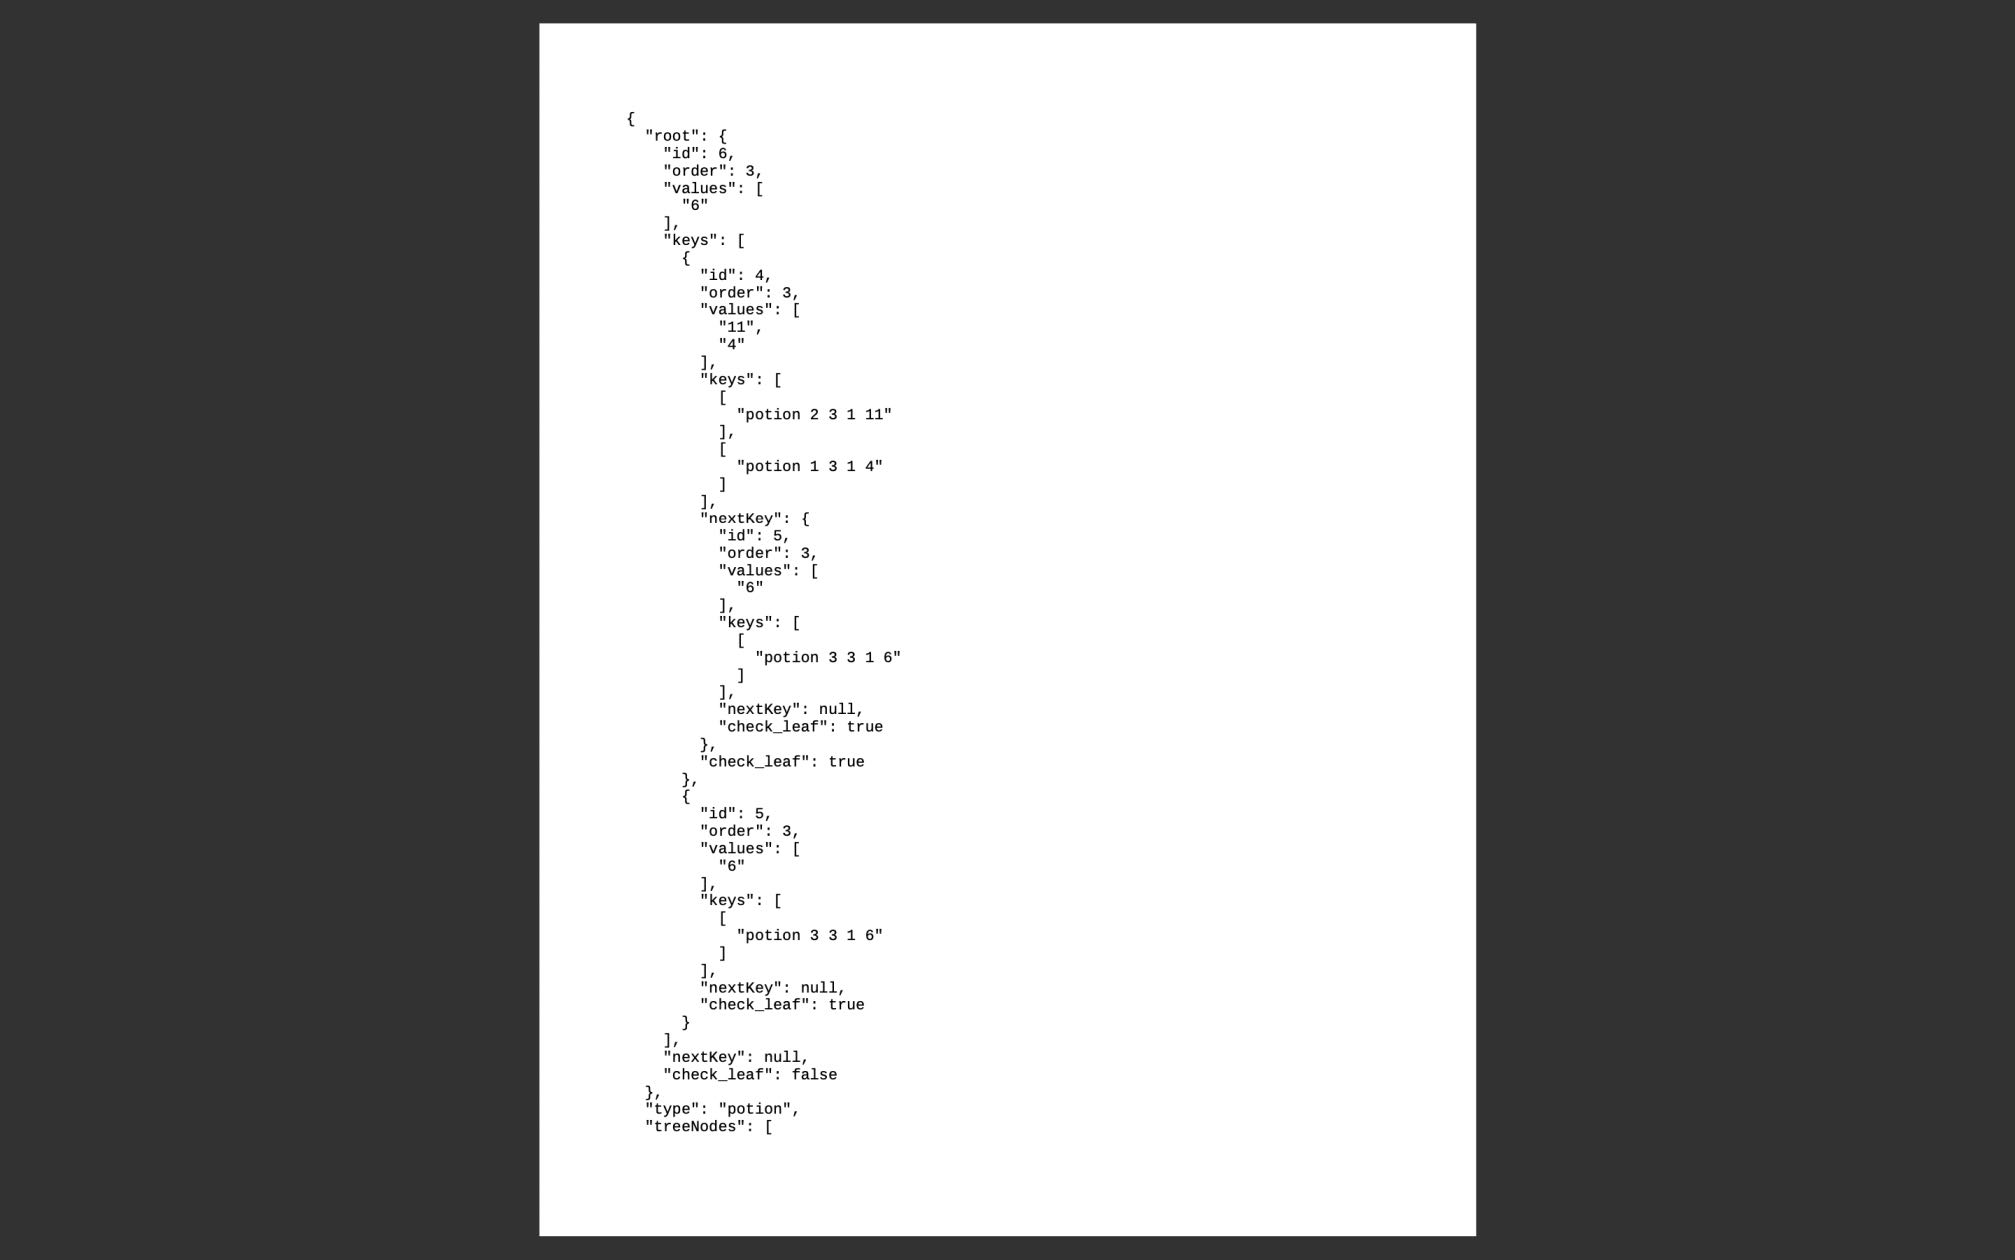
\includegraphics[width=.8\textwidth]{figures/bplus.jpg}
    \caption{bplus\_potion.json (not entire file because it is too long)}
\end{figure}
\begin{figure}[H]
    \centering
    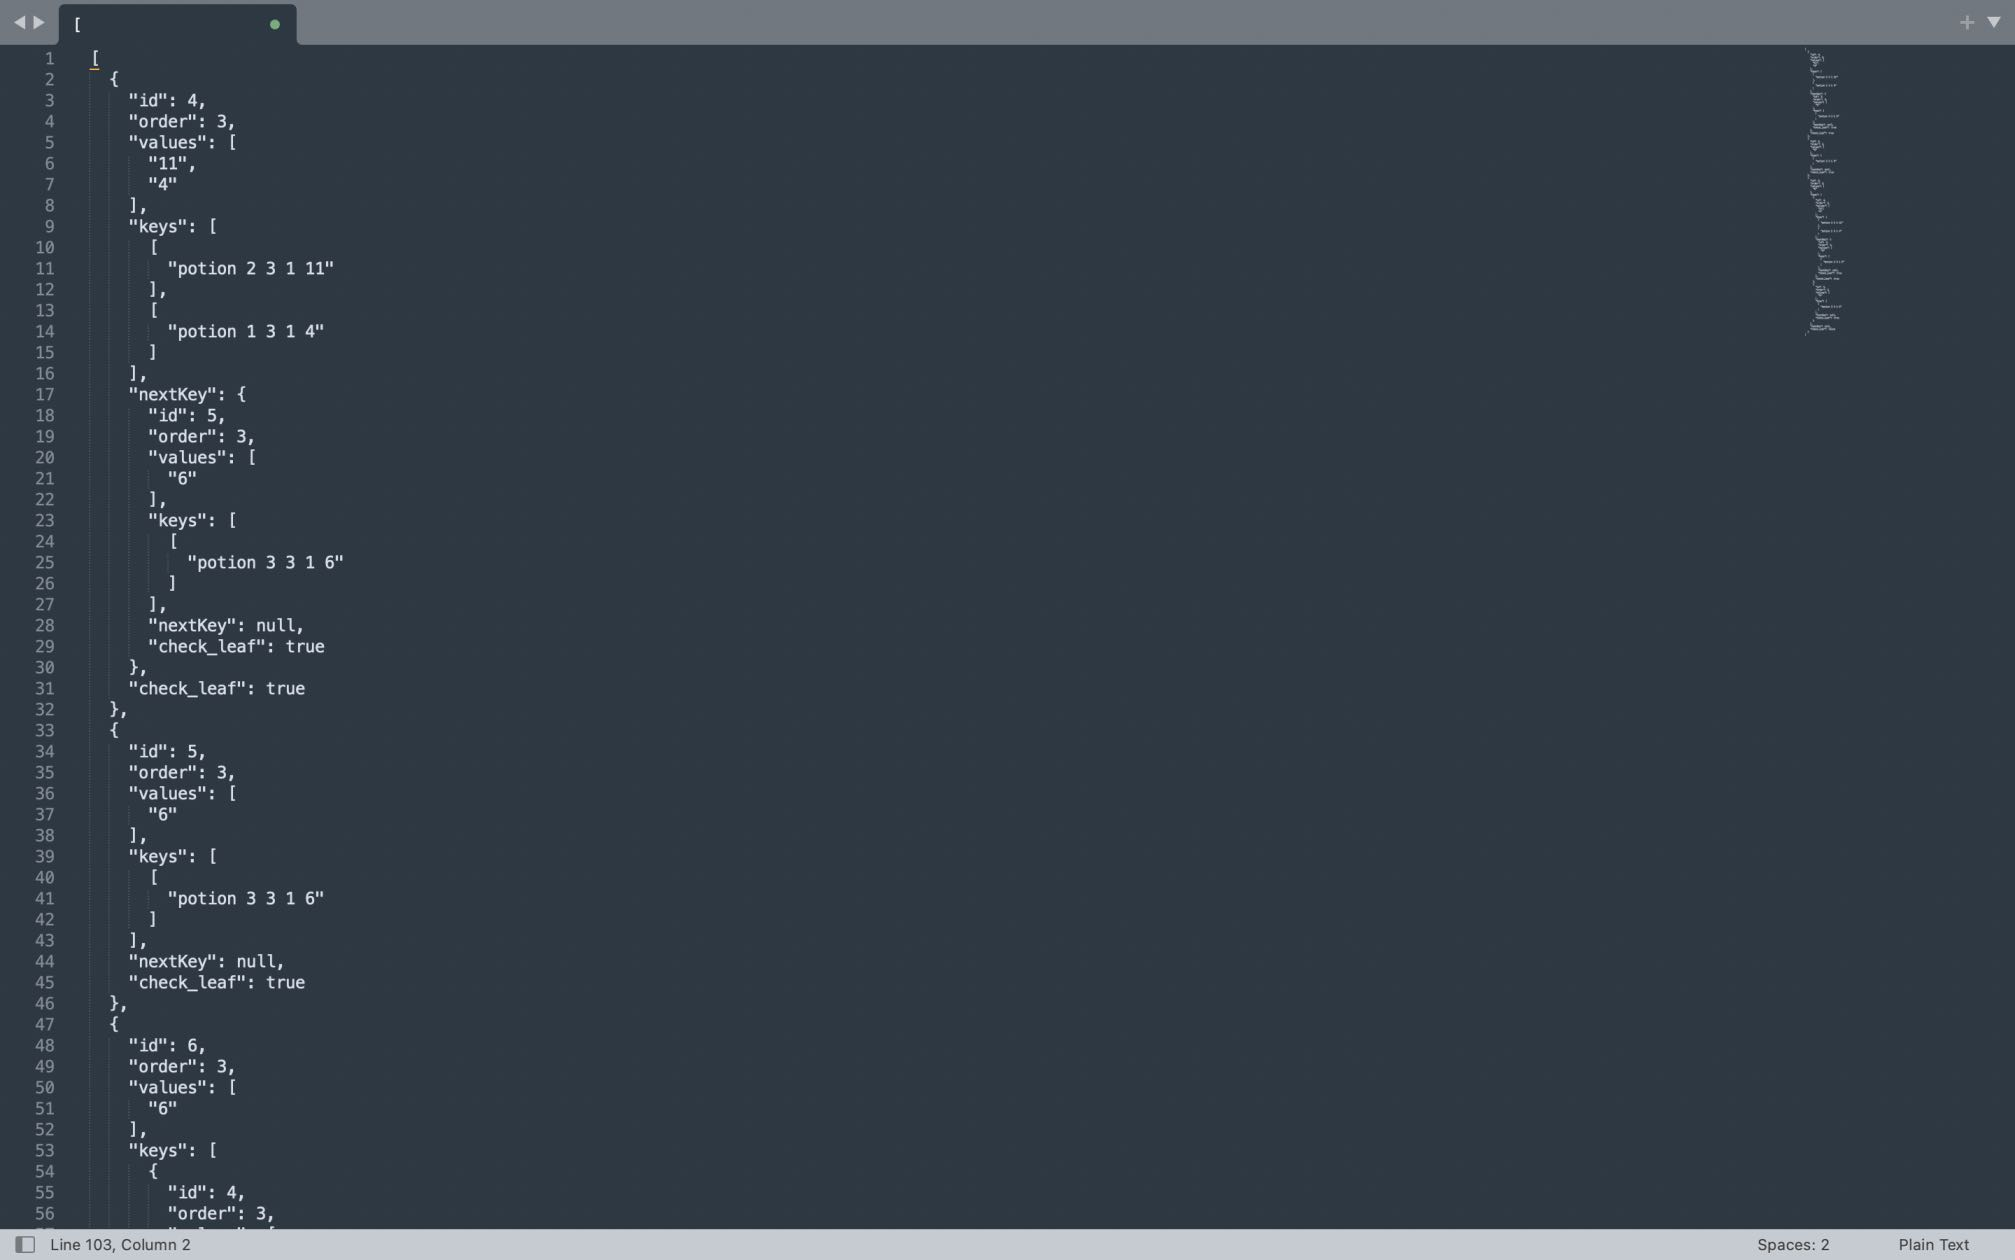
\includegraphics[width=.8\textwidth]{figures/node.jpg}
    \caption{nodes\_potion.json (not entire file because it is too long)}
\end{figure}
\begin{figure}[H]
    \centering
    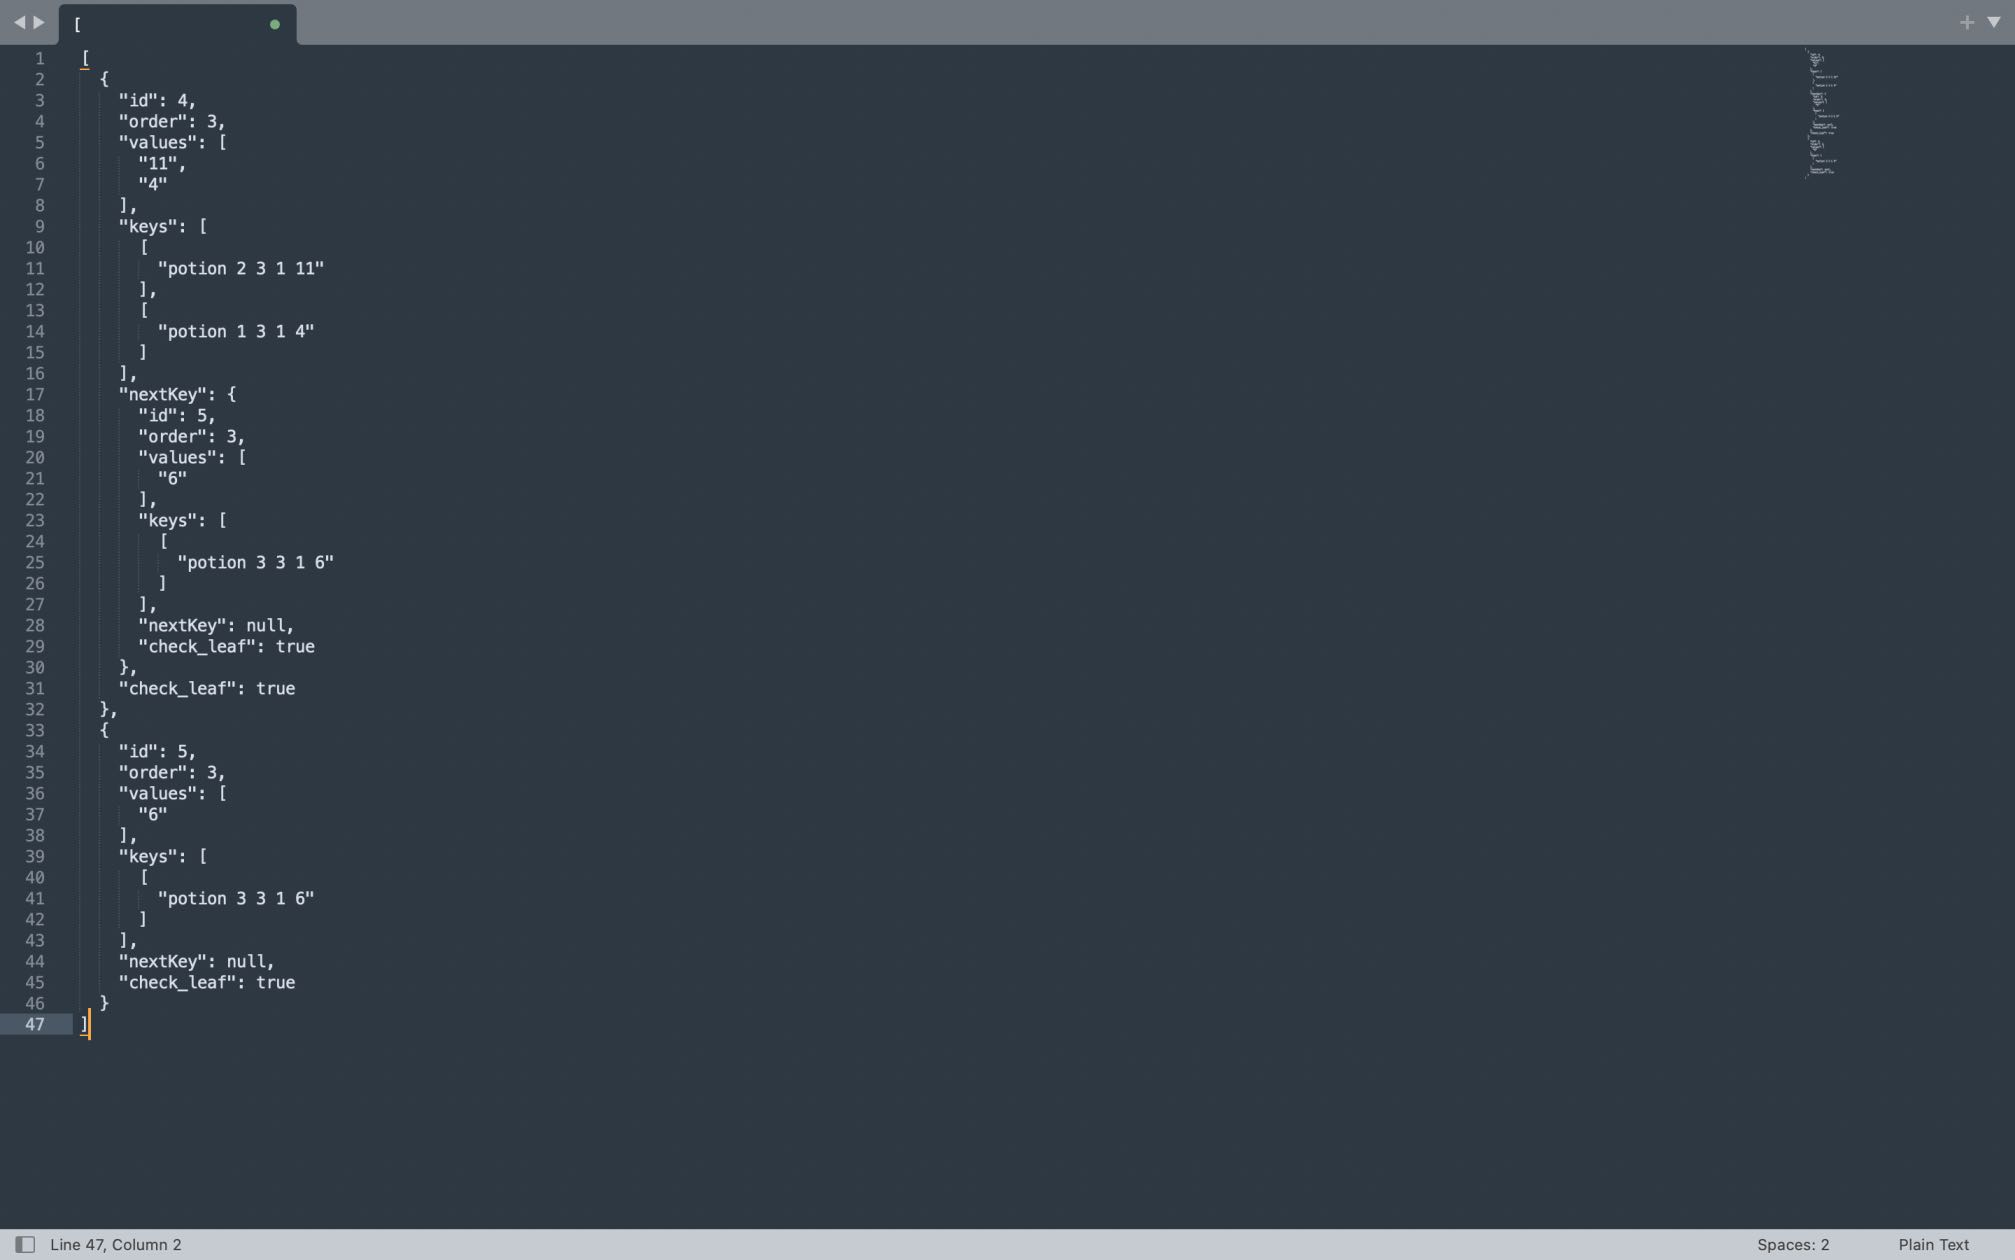
\includegraphics[width=.8\textwidth]{figures/parent_keys.jpg}
    \caption{parent\_keys\_potion.json }
\end{figure}
\begin{figure}[H]
    \centering
    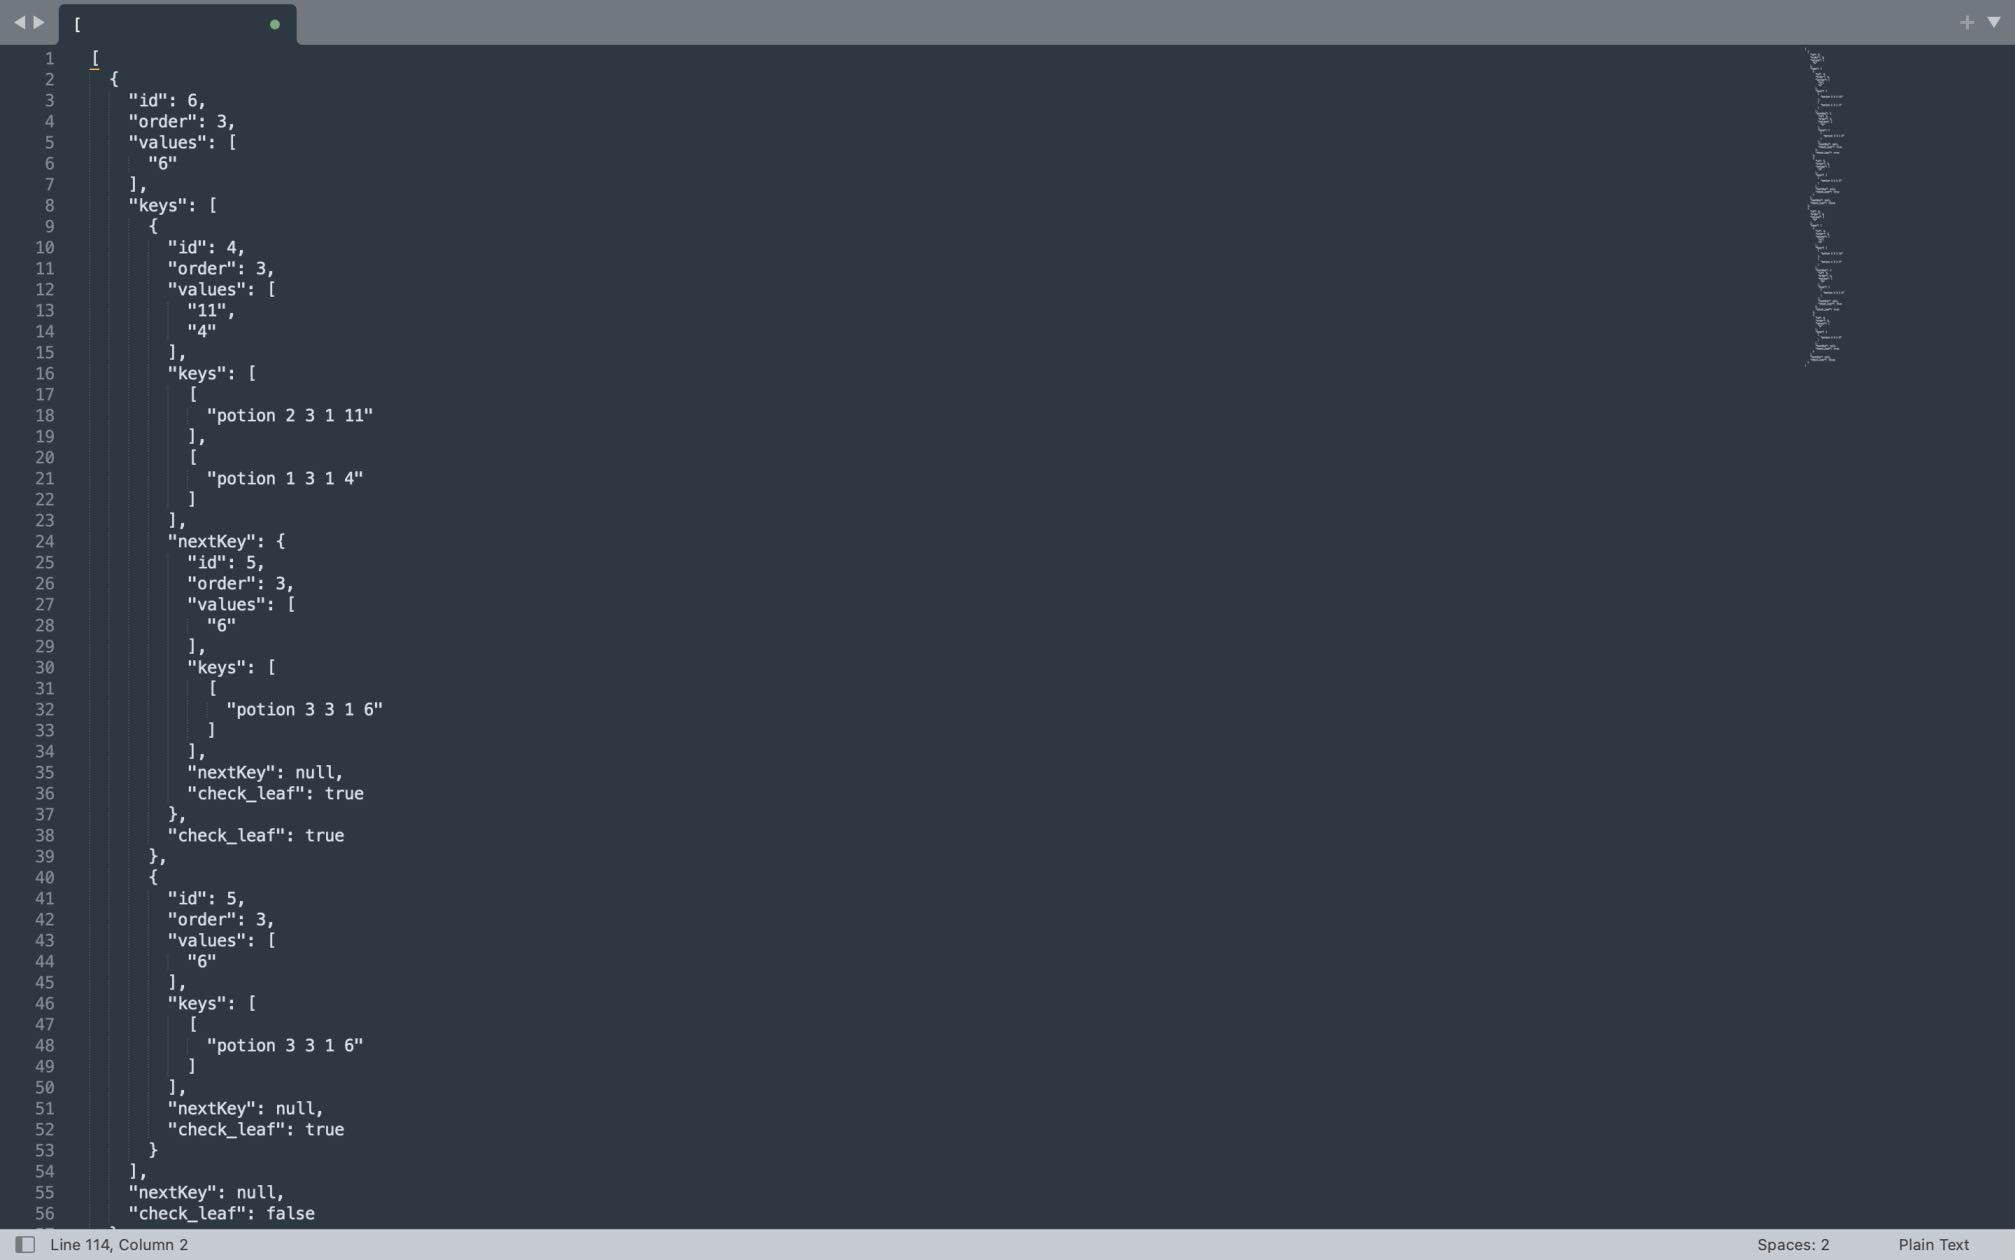
\includegraphics[width=.8\textwidth]{figures/parent_values.jpg}
    \caption{parent\_values\_potion.json (not entire file because it is too long)}
\end{figure}

\section{Operations}
\label{sec:operations}
Write your DDL and DML operations by referring to the structures in your design.

\subsection{HALO Definition Language Operations}

\subsection{HALO Manipulation Language Operations}

\section{Conclusion \& Assessment}
\label{sec:conclusion}
In this project we have used B+ structure from https://www.programiz.com/dsa/b-plus-tree. However, we have changed most of the parts because it does not satisfy the requirements. Most challenging part of the project is storing the B+ tree in a json file and get the tree from the json file. The first implementation of tree cause cyclic loop while storing them as json file because all nodes contains attribute next\_keys which contains nodes. We solve this issue by using recursion and create different parent dictionary. For design part of the project we keep our design simple. We use basic headers and system catalog. Our design allow us to find the required page in fastest way then in a page find the record. Although the structure is simple, it is very efficient to search, list and filter data with B+ Tree indexing. However, creating and deleting a record with B+ Tree indexing is little costly because it needs many operations to find the correct index and arrange the nodes again. 
\end{document}
